\documentclass[a4paper,11pt]{article}
\usepackage{layout}
\usepackage{lscape}
\usepackage[utf8]{inputenc}
\usepackage{a4wide}
\usepackage[dvips]{graphicx}
\usepackage{url}
\usepackage[colorlinks=true]{hyperref}
\usepackage[table,dvipsnames]{xcolor}[2004/07/04]

\author{Jachym Cepicky}

\title{Implementation of OGC's WPS standard: PyWPS}

\makeatletter
%\Lesejk
\def\Lesejk{{\tt{}Les-e\makebox(2,11)[t]{\rotatebox{35}{j}}\kern-.1667em\lower.5ex\hbox{\rotatebox{315}{k}}\kern-.125em\@}}


\newcommand{\link}[1]{\texttt{<\url{#1}>}}
\newcommand{\pywpssite}{\url{http://pywps.wald.intevation.org}}
\newcommand{\pywpswiki}{\url{http://pywps.ominiverdi.org}}
\newcommand{\note}[1]{\medskip{}\noindent{}NOTE: #1\medskip{}}
\newcommand{\version}{\emph{2.0.0}}
\makeatother


\pagestyle{plain}

\begin{document}
\maketitle{}

\bigskip
\begin{quote}
    Copyright \copyright  2006 PyWPS Development Team
    Permission is granted to copy, distribute and/or modify this document
    under the terms of the GNU Free Documentation License, Version 1.2
    or any later version published by the Free Software Foundation;
    with no Invariant Sections, no Front-Cover Texts, and no Back-Cover Texts.
    A copy of the license is included in the section entitled "GNU
    Free Documentation License".
\end{quote}
\bigskip


In this file, you can found the description of installation and
configuration of PyWPS script. At the and, you can learn, how to add
your own process to the list of processes. The file describes most recent
version of PyWPS (\version), available in subversion respository.

PyPWS project has been started on April 2006 with support of DBU --
Deutsche Bundesstiftung Umwelt (\url{http://dbu.de}) and with help of
GDF-Hannover (\url{http://gdf-hannover.de}) and Help Service Remote
Sensing (\url{http://www.bnhelp.cz}) companies. Initial author is Jachym
Cepicky (\url{http://les-ejk.cz}).
    

    \tableofcontents

\newpage

%---------------------------------------------------------------------
\section{Introduction}
PyWPS (Python Web Processing Service) is implementation of Web
Processing Service standard from Open Geospatial Consortium.

It has been started on Mai 2006 as project supported by DBU. It offers
environment for programming own process (geofunctions or models) which can
be accessed from the public. The main advantage of PyWPS is, that it has
been written with native support for GRASS. Access GRASS modules via web
interace should be as easy as possible.

Processes can be written using GRASS GIS, but usage of other programs is
also possible. Usage together with R package or GDAL or PROJ tools.

PyWPS is written in Python programming language, your processes must use
this language too. 

PyWPS Homepage can be found at \pywpssite.
PyWPS Wiki is hosted on \pywpswiki. 

\subsection{How it works}
PyWPS is an translator application between client (Web Browser, Desktop
GIS, command line tool, \dots) and working tool installed on the server.
PyWPS does no work by it self. As working tool, GRASS GIS, GDAL, PROJ, R
and other programs can be used.

\begin{figure}[ht]
\begin{center}
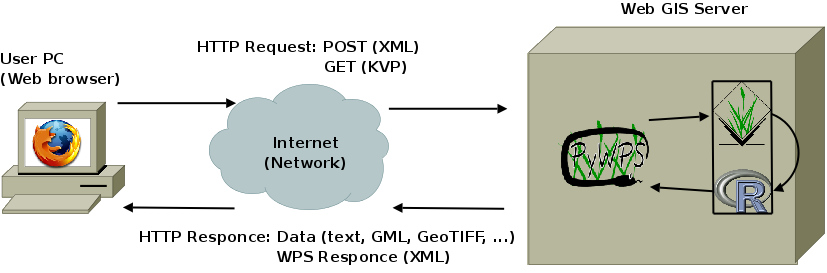
\includegraphics[width=1\textwidth]{pic/pywps-schema}
\caption{How does PyWPS work: GRASS GIS is in this case working tool}
\label{pic:pywps}
\end{center}
\end{figure}

%---------------------------------------------------------------------
\section{Quick install}
\begin{enumerate}
    \item Install PyWPS, see page~\pageref{install} for details
    \item NOTE: Copy original files (process examples, configuration files)
    with \texttt{.py-dist} suffix to \texttt{.py}, when you see them.
    \item Edit configuration files in \texttt{pywps/etc/} directory. See
    page~\pageref{configuration} for details.
    \item Create or edit \texttt{\_\_init\_\_.py} file in
    \texttt{pywps/processes} directory. Add available process names to
    \texttt{\_\_all\_\_} structure.
    \item Add your processes to \texttt{pywps/processes} directory. See
    page~\pageref{processes} for details.
    \item Run PyWPS with \texttt{./wps.py} command, see
    page~\pageref{testing} for details.
\end{enumerate}

    
%---------------------------------------------------------------------
\section{Know issues}
Known bugs and limitations to \date
\begin{itemize}
\item Sometimes, when there is e.g. SyntaxError in the process, teporary file \texttt{/tmp/pywps*} is not deleted, which ledts to \texttt{ServerBussy} exception and the files have to be removed by hand.
\item  If inputs are of type \texttt{LiteralValue} and it's type is
string, it is not controlled properly. Take care on your inputs and do
not use it directly in scripts to avoid your server to be hacked.
\end{itemize}

Please report all problems or unexpected handeling either via pywps mailing
list\footnote{\href{http://wald.intevation.org/mailman/listinfo/pywps-devel}{PyWPS
- development list}}
or using PyWPS
bugtracker\footnote{\href{http://wald.intevation.org/tracker/?atid=174&group\_id=22&func=browse}{PyWPS
Bug tracker}}.

%---------------------------------------------------------------------
\section{Installation}
\label{install}   
Required packages:
    
\begin{itemize}
    \item python 
    \item python-xml 
\end{itemize}
    
Recommended packages:
    
\begin{itemize}
    \item Web Server (e.g. Apache) -- \url{http://httpd.apache.org} -  You
    will need an web server, to be able to execute processes from remote
    computers.

    \item GIS GRASS  -- \url{http://grass.itc.it} - Geographical Resources
    Analysis Support System (GRASS) is Open Source GIS, which provides more
    then 350 modules for raster and vector (2D, 3D) data analysis. PyWPS is
    written with native support for GRASS and it's functions.

    \item PROJ.4  -- \url{http://proj.maptools.org} - Cartographic
    Projections library used in various Open Source projects, such as
    GRASS, UMN MapServer, QGIS and others. It can be used e.g. for data
    transformation.

    \item GDAL/OGR  -- \url{http://gdal.org} - translator library for
    raster geospatial data formats, is used in various projects for
    importing, exporting and transformation between various raster and vector
    data formats.

    \item R  -- \url{http://www.r-project.org} - is a language and environment
    for statistical computing and graphics.

\end{itemize}
    
\subsection{Installation the quick 'n' dirty way}
For installing pywps to your server simply unzip the archive to the
directory, where cgi programs are allowed to run. You can also use current
repository version.

\begin{verbatim}
$ cd /usr/lib/cgi-bin/
$ tar xvzf /tmp/pywps-VERSION.tar.gz
$ pywps/wps.py
\end{verbatim}

\subsection{Installation the 'clean' way}
Unzip the package 
\begin{verbatim}
$ tar -xzf pywps-VERSION.tar.gz
\end{verbatim}
and run 
\begin{verbatim}
$ python setup.py install
\end{verbatim} 

Several binary packages for Linux distributios are also avaliable on PyWPS
site\footnote{\pywpssite}.

%---------------------------------------------------------------------
\section{Configuration}
\label{configuration}
    
Before you start to tune your pywps program, you should get your copy of
OpenGIS(R) Web Processing Service document (OGC 05-007r4) version 0.4.0
from\\ \url{http://www.opengeospatial.org/specs/?page=specs}
    
\note{Note, that the configuration option are CASE SENSITIVE}
    
Pywps configuration takes places in two files. The files are actually python
scripts, so it does not harm, if you have some experience in python
programming language. But you should be able to setup the program without
any python knowledge.

The first file is in \texttt{etc/settings.py} and (optional) the second file is
\texttt{etc/grass.py} which has to be setuped if you do want to use
GRASS GIS modules in your scripts. Some special "tuning" can be done in \texttt{processes/\_\_init\_\_.py}
file. You can allways obtain original configuration files from
\texttt{Wps/default\_settings.py} and \texttt{Wps/default\_grass.py}.
    
\subsection{\texttt{etc/settings.py}}
    
This file has got two sections: WPS and serverSettings
    
In the \texttt{WPS} section, the main configuration is set, which appears mostly in
GetCapabilities request. The \emph{mandatory} parameters, which should be set up
are (with default/recommend values):
    

\begin{verbatim}
WPS = {
    'version': "0.4.0",
    'ServiceIdentification': {
        'Title':"Jachym's WPS server",
        'ServiceType':"WPS",
        'ServiceTypeVersion':"0.1.0",
        'Abstract':'Abstract to this WPS',
    },
    'ServiceProvider': {
            'ProviderName' : "Your Company",
            'IndividualName':"Your Name",
            'PositionName':"Your Position",
            'Role':"your role",
            'DeliveryPoint': "Street",
            'City': "City",
            'PostalCode':"00000",
            'Country': "Your country",
            'ElectronicMailAddress':"your.email@address",
    },

    'OperationsMetadata': {
        'ServerAddress' : "http://localhost/cgi-bin/wps/wps.py",
    },
    'Keywords' : ['GRASS','GIS','WPS'],
}
\end{verbatim}

    
In the \texttt{ServerSettings} section, the variables are set, which have impact on
the whole server.
    

\begin{verbatim}
ServerSettings = {
        # NOTE: You have to create this directory manually and set rights, so
        #       the program is able to store data in there 
        'outputPath': '/var/www/wpsoutputs',
        
        #
        # 'outputUrl' - URL of the directory, where the outputs will be stored
        'outputUrl':  'http://192.168.1.31/wpsoutputs',
        
        #
        # tempPath - path to directory, where temporary data will be stored.
        # NOTE: the pywps has to have rights, to create directories and files
        #       in this directory
        'tempPath': '/tmp',
        
        #
        # maxOperations - maximum number of operations, which is allowed to low
        # on this server at ones 
        # default = 1
        'maxOperations':1,
        
        #
        # maxSize: maximum input file size in bytes
        # NOTE: maximum file size is 5MB, no care, if this number is higher
        'maxSize':5242880, # 5 MB
        
        #
        # maxInputParamLength: maximal length of input values
        # NOTE: maximum length of input parameters is 256, no matter, how height
        #       is this number
        'maxInputParamLength':256,
}
\end{verbatim}


\subsection{\texttt{etc/grass.py}}
    
This file servers for configuration of GRASS GIS environment (if your
processes need one). Everything is stored in \texttt{grassenv} structure. 
    

\begin{verbatim}
grassenv = {
    # PATH in which your modules (processes) should be able the search.
    # Default value:
    'PATH': "/usr/local/grass-6.1.cvs/bin/:/usr/local/grass-6.1.cvs/scripts/:\
    /usr/bin/:/bin/:",
    
    # Add eventually some other path, in which should GRASS search for modules
    'GRASS_ADDON_PATH': "",
    
    # Version of GRASS, you are using
    'GRASS_VERSION': "6.1.cvs",
    
    # GRASS_PERL, where is your PERL bin installed
    'GRASS_PERL': "/usr/bin/perl",
    
    # GRASS_GUI should be always "text" unless you know, what you are doing
    'GRASS_GUI': "text",
    
    # GISBASE is place, where your GRASS installation is
    'GISBASE': "/usr/local/grass-6.1.cvs",
    
    # LD_LIBRARY_PATH
    'LD_LIBRARY_PATH':"/usr/local/grass-6.1.cvs/lib",
    
    # HOME has to be set
    'HOME':"/var/www",
}
\end{verbatim}



\subsection{Testing after installation}
\label{testing}
For test, just run
\texttt{wps.py} in your command line:
    
\begin{verbatim}
$ ./wps.py
Content-type: text/xml

<?xml version="1.0" ?>
<ExceptionReport version="1.0.0" xmlns="http://www.opengis.net/ows" 
        xmlns:xsi="http://www.w3.org/2001/XMLSchema-instance">
        <Exception exceptionCode="MissingParameterValue" locator="request"/>
</ExceptionReport>
    \end{verbatim}

     
If you got some other message, like e.g.:
     

    \begin{verbatim}
Traceback (most recent call last):
  File "trunk/index.py", line 53, in ?
    from Wps import wpsexceptions
  File "/home/jachym/prog/pywps/trunk/Wps/wpsexceptions.py", line 8, in ?
    from xml.dom.minidom import Document
ImportError: No module named xml.dom.minidom
    \end{verbatim}

     
Than something is wrong with your Python installation or with the program.
This message means, that the xml.dom.minidom package is not installed in
your system.
     


    
%---------------------------------------------------------------------
\section{Add your own processes}
\label{processes}
\note{This section has changed from previous stable 1.0.0 version. The
processes, you defined for 1.0.0 branch should work for 2.0.0 branch too.}
    
All processes are stored in the \texttt{processes} directory. Put your file
e.g. \texttt{myprocess.py} in there. Several example processes are
distributed along with PyWPS source code.
    
Process is python class derived from prepared \texttt{WPSProcess} class in
\texttt{pywps.Wps} package. In it \texttt{\_\_init\_\_(self)} method,
process metadata, inputs and outpus are defined and in
\texttt{execute(self)} method, own computation is performed.


It is possible also to add as many your functions, as you wish.
    
\subsection{Process initialization and configuration}
First of all, you have to add name of your process to
\texttt{pywps/processes/\_\_init\_\_.py} file. Then you can start to edit
the process file it's self.

\begin{verbatim}
01 # importing necessary files
02 import pywps.Wps.WPSProcess
03 
04 class Process(WPSProcess):
05      def __init__(self):
06          WPSProcess.__init__(self,
07                Identifier="ogr2ogr",
18                Title="ogr2ogr interface",
19                Abstract="Convert vector file to another format",
10                processVersion = "0.2",
11                statusSupported="true",
12                storeSupported="true")
\end{verbatim}

We defined new process called \texttt{ogr2ogr}. The process is allowed to
store it's output data on the server (\texttt{storeSupported}) and it is also possible to run it in
asynchronous mode (\texttt{statusSupported}).
     
Eventually optional attributes can be found in the table 38 - "Parts of
ExecuteResponse data structure" in the WPS reference
document\footnote{\url{http://www.opengeospatial.org/standards/requests/28}}. It is also possible to redefine some
variable later, after initialization:

\begin{verbatim}
13
14          self.Title="ogr2ogr interface"
15
\end{verbatim}


\paragraph{Metadata defition} is stored in array \texttt{self.Metadata} in
\texttt{\_\_init\_\_} method. You can add new Medatada using
\texttt{self.AddMetadata()} method:
\begin{verbatim}
            self.AddMetadata(Identifier="point",type="point",
                            textContent="Click in the map")
\end{verbatim}

This code will produce in DescribeProcess responce document following
element:
\begin{verbatim}
...
<ows:Metadata Identifier="point" type="point">
    Click in the map
</ows:Metadata>
...
\end{verbatim}

\subsubsection{Data Inputs}
Data inputs are stored in \texttt{self.Inputs} array. To add inputs to
your process, you should use methods defined in \texttt{WPSProcess} class.

Four types of data inputs are defined:
\begin{itemize}
    \item Literal Input -- Basic literal input -- single number or text
    value
    \item ComplexValue Input  -- Mostly vector file embded in input XML
    request
    \item ComplexValueReference Input -- URL to location, where the process
    is supposed to get the input data.
    \item BoundingBox Input -- Coordinates for lower-left and upper-right
    corner.
\end{itemize}

ComplexValue and ComplexValueReference defined on the same way -- PyWPS is
able to guess, if the input data are reference (link) to some map or raw
data directly.

\paragraph{LiteralInput}

Basic type of data input is \texttt{LiteralInput} type. To define
LiteralInput the easy way, you should use \texttt{AddLiteralInput} method:

\begin{verbatim}
20
21          self.AddLiteralInput(Identifier="value",
                                 Title="Value to be added",
                                 type=type(0))
\end{verbatim}

Above example will add new input with identifier \texttt{value} of type
integer. Examples of other possibilities of LiteralInputs and resulting
part of XML are folowing:

\subparagraph{Example of any allowed input value (default)}
\begin{verbatim}
self.AddLiteralInput(Identifier="someinput", 
                     Title="Some Input", 
                     allowedvalues='*')

...
  <Input>
    <ows:Identifier>someinput</ows:Identifier>
    <ows:Title>Some Input</ows:Title>
    <ows:Abstract/>
        <LiteralData>
            <SupportedUOMs defaultUOM="m">
                <ows:UOM>m</ows:UOM>
            </SupportedUOMs>
            <ows:AnyValue/>
        </LiteralData>
    <MinimumOccurs>1</MinimumOccurs>
  </Input>
...
\end{verbatim}

\subparagraph{Example of specified list (with range) of allowed inputs}

Following example will define input with specified list of values: Only
values 20, 30, everything between 40-100 and 110 will be accepted:
\begin{verbatim}
self.AddLiteralInput(Identifier="someinput",
                     Title="Some Input",
                     allowedvalues=[20,30,[40,100],110])

...
  <Input>
    <ows:Identifier>someinput</ows:Identifier>
    <ows:Title>Some Input</ows:Title>
    <ows:Abstract/>
    <LiteralData>
    	<SupportedUOMs defaultUOM="m">
        <ows:UOM>m</ows:UOM>
        </SupportedUOMs>
        <AllowedValues>
            <Value>20</Value>
            <Value>30</Value>
            <Range>
                <MinimumValue>40</MinimumValue>
                <MaximumValue>100</MaximumValue>
            </Range>
            <Value>110</Value>
        </AllowedValues>
    </LiteralData>
    <MinimumOccurs>1</MinimumOccurs>
  </Input>
...
\end{verbatim}

For further documentation, refere example processes distributed with the
source code as well as \texttt{pydoc~pywps/wps/process.py}. This help is
also available in
\texttt{process.html}\footnote{\href{http://wald.intevation.org/plugins/scmsvn/viewcvs.php/*checkout*/trunk/doc/process.html?rev=369&root=pywps}{Documentation
to process.py module}} file distributed along with PyWPS
source code.

\paragraph{ComplexInput}
If the request comes as HTTP GET, it is assumed, that the input is only
reference to some map. If it comes as HTTP POST, PyWPS tryes to guess, if
the client is sending URL to source of the data or if the input data are
part of input XML request (e.g. as GML file). So, you, as a process coder
do not have to take care on this:

\begin{verbatim}
self.AddComplexInput(Indentifier="inputmap",
      Title="Input map, which should be processed",
      Formats=["text/xml","image/tiff"])
...
    <Input>
        <ows:Identifier>input</ows:Identifier>
        <ows:Title>Input raster map</ows:Title>
        <ows:Abstract/>
        <ComplexData defaultFormat="image/tiff">
            <SupportedComplexData>
                <Format>image/tiff</Format>
                <Format>text/xml</Format>
            </SupportedComplexData>
        </ComplexData>
        <MinimumOccurs>1</MinimumOccurs>
    </Input>
\end{verbatim}

\paragraph{BoundingBox Input}
With bounding box, you can define two coordinate pairs, if you have to.

\begin{verbatim}
self.AddBondingBoxInput(Identifier="bbox",
        Title="BBox input")
\end{verbatim}

\subsubsection{Data Outputs}
Again four types of output are defined:
\begin{itemize}
    \item Literal Output
    \item ComplexValue Output
    \item ComplexValue Reference
    \item BoundingBox Output
\end{itemize}
    
Data outputs can be defined on similar way, using similar methods:

\paragraph{LiteralOutput}
\begin{verbatim}
self.AddLiteralOutput(Identifier="litoutput",
                     Title="Resulting output value")

...
  <Output>
    <ows:Identifier>litoutput</ows:Identifier>
    <ows:Title>Resulting output value</ows:Title>
    <ows:Abstract/>
    <LiteralOutput>
      <SupportedUOMs defaultUOM="m">
        <ows:UOM>m</ows:UOM>
      </SupportedUOMs>
    </LiteralOutput>
  </Output>
...
\end{verbatim}

\paragraph{ComplexValue and ComplexValueReference Output}
To the oposite of data Inputs, Outputs can distinguish between ComplexValue
output and ComplexValueReference. ComplexValue is directly embed into the
output XML document and ComplexValueReference is stored on the server and
only URL pointing the the file is refering to it. In general, vector files
in GML format can be easy embed to the output XML, TIFF raster files is
better to leave on the server.

\begin{verbatim}
self.AddComplexReferenceOutput(Identifier="output",
                Title="Resulting output map",
                Formats=["image/tiff"])

...
  <Output>
    <ows:Identifier>output</ows:Identifier>
    <ows:Title>Resulting output map</ows:Title>
    <ows:Abstract/>
    <ComplexOutput defaultFormat="image/tiff">
      <SupportedComplexData>
        <Format>image/tiff</Format>
      </SupportedComplexData>
    </ComplexOutput>
  </Output>
...
\end{verbatim}

\paragraph{BoundingBox Output}
Beside LiteralValue and ComplexValue, BoundingBoxValue is also defined. 
The coordinates are stored in array of four members:

\begin{verbatim}
self.GetInputValue("bboxinput")
[0,0,100,100]
\end{verbatim}

\bigskip

So on our \texttt{ogr2ogr} process, we have to define three types of input:
\texttt{ComplexValue} of input vector file and EPSG codes of target and
source files:

\begin{verbatim}
16      self.AddComplexInput(Identifier="inputmap",
17          Title ="Input vector file",
18          Abstract = "Input vector file to be converted",
19          Formats=["text/xml"])
20
21      self.AddLiteralInput(Identifier="sepsg",
22          Title="Source EPSG",
23          Abstract="Source EPSG code",
24          value=4326) 
\end{verbatim}


And we also define two outputs: ComplexValueReference and ComplexValue
type.


\begin{verbatim}
25      self.AddComplexOutput(Identifier="outputmap",
26          Title ="Input vector file",
27          Abstract = "Input vector file to be converted",
28
29      self.LiteralOutput(Identifier="sepsg",
30          Title="Source EPSG",
31          Abstract="Source EPSG code",
32          value=4326) 
\end{verbatim}


\subsection{Process Programming}
    
The process must be defined in the \texttt{execute(self)} function. You can
access the input values via \texttt{self.GetInputValue(Identifier)} method.

\note{Usage of the old method, accessing the values via
\texttt{self.Inputs[index]['value']} or via \texttt{self.DataInputs} array
is possible, but should not be used.}

Also variable \texttt{self.grassenv} will be in your process at your
service. This dictionary stores environment variables used by GRASS GIS,
such se \texttt{LOCATION\_NAME} or \texttt{MAPSET}.

Output values should be set using \texttt{self.SetOutputValue(Identifier,
value)} method.

\note{Usage of the old methods of output values setting, directly to 
\texttt{self.Outputs[index]['value']} variable or to
\texttt{self.DataOutputs['identifier']} dictionary, is possible, but should
better not be used.}

If you need to execute some shell command, you should use
\texttt{self.Cmd(command,["string for standard input"])} instead of e.g.
\texttt{os.system()} or \texttt{os.popen()} functions.


\begin{verbatim}
33
35      def execute(self):
36          
37          #
38          # calculation
39          #
30          self.Cmd("""ogr2ogr -s_srs "+init=epsg:4326" -t_srs \
31          "+init=epsg:2065" %s output.file""" % (self.GetInputValue("inputmap")))
32         #
43         # setting results
44         #
45         self.SetOutputValue("outputmap","output.file")
46         self.SetOutputValue("sepsg","4326")
47
48         return
\end{verbatim}

\subsubsection{Error handling}
    
At the end of the \texttt{execute} function, \texttt{None} value should be returned. Any other 
value means, that the calculation will be stopped and error report will be returned back to the client.
    

\subsubsection{Using standard in- and output with external commands}
The \texttt{self.Cmd()} accepts \texttt{input} parameter, wich is a text
string, which is directred to standard input of the command:

\begin{verbatim}
    result = self.Cmd(cmd="wc -c",
             input="calculate number of characters for this sentence")

    # result[0].split()
\end{verbatim}

\texttt{self.Cmd()} returns list of lines from the programms standard
output to the process:

\begin{verbatim}

    for line in self.Cmd("ls -l"):
        # do some operations of list of files
        pass
\end{verbatim}


\subsection{GRASS specific notes}

Special class for GRASS GIS is defined too, which has functions and
variables specific to this program. The process, in which should use GRASS
modules should be defined as follows:

\begin{verbatim}
# importing necessary files
import pywps.Wps.GRASSWPSProcess

class Process(GRASSWPSProcess):
     def __init__(self):
         GRASSWPSProcess.__init__(self,
               Identifier="spearpath",
               Title="Spearfish path searching",
               Abstract="Find the shortest path on the roads map on Spearfish dataset",
               processVersion = "0.2",
               statusSupported="true",
               storeSupported="true",
               # grassLocation="/var/www/spearfish60/" # work on existing location)
\end{verbatim}

By default, \texttt{self.grassLocation}\footnote{See e.g.
\href{http://grass.itc.it/grass63/manuals/html63\_user/helptext.html}{GRASS
manual} for details} 
 variable is set to \texttt{None},
which means, that temporary location will be created and after the
calculation is done, it will be deleted again. You can set this while
process initialization or
later\footnote{\texttt{self.grassLocation="/path/to/location"}}.

    
\texttt{WPSProcess} class provides special method
\texttt{self.GCmd(command\_string)}, which tryes to catch output from GRASS
modules, especially progress information inidcated by percent done. Method
\texttt{GCmd()} stores the output of GRASS modules to \texttt{self.status}
variable, so if the process is running assynchronously, client application
can track the progress of each module directly.

\begin{verbatim}
    def execute(self):
        """
        This function serves like simple GRASS - python script

        It returns None, if process succeed or String if process failed
        """
        self.GCmd("g.region -d")


        # v.net.path reads from standard input
        self.GCmd("v.net.path in=roads out=path","0 %s %s %s %s" % (self.GetInputValue('x1'),
                self.GetInputValue('y1'),
                self.GetInputValue('x2'),
                self.GetInputValue('y2')))

        self.GCmd("v.out.ogr format=GML input=path dsn=out.xml olayer=path.xml")

        if "out.xml" in os.listdir(os.curdir):
            shutil.copy("out.xml","out2.xml")
            self.SetOutputValue('outputReference',"out.xml")
            self.SetOutputValue('outputData',"out2.xml")
            return
        else:
            return "Ouput file not created!"
\end{verbatim}

%---------------------------------------------------------------------

It is also possible to run GRASS modules using python's
\texttt{os.system()} or \texttt{os.popen()} function.  Before you do so, it
is important to import the \texttt{os} python package (usually one of the
first lines in the file). This approach might not be the best, but it is
the simplest one. Feel free to use any other low-end functions.
    
    
Unfortunately, the GRASS modules are very verbose. Some messages are
written to STDOUT, some to STDERR. The STDERR will be stored in the error
file of your web server. But you have to "catch" the messages, sent to
STDOUT. This can be done e.g. by using "$1>\&2$" statement (redirecting
STDOUT to STDERR in shell):

\begin{verbatim}
os.system("""
    echo "Rekni jim drazi, tatko, za to nic nedas."  >&2
""")
\end{verbatim}

You can avoid this problem using formentioned \texttt{self.GCmd()} method.


%---------------------------------------------------------------------
\section{Testing your new process}

To test your PyWPS installation, you run it either as Webserver
cgi-application or in the command line directly. It is always good to start
with the command line test, so do not have to check \texttt{error.log} of
the web server.

\begin{itemize}
    \item GetCapabilities request (webserver)
\begin{verbatim}
./wps.py "service=wps&request=getcapabilities"

wget -nv -q -O - "http://localhost/cgi-bin/wps.py?\
    service=Wps&request=getcapabilities"
\end{verbatim}
        
    \item DescribeProcess request:
\begin{verbatim}
./wps.py "version=0.4.0&service=Wps&request=DescribeProcess&\
    Identifier=your_process"

wget -nv -q -O - "http://localhost/cgi-bin/wps.py?\
    version=0.4.0&service=Wps&request=DescribeProcess&\
    Identifier=your_process"
\end{verbatim}
        
    \item Execute request:
\begin{verbatim}
./wps.py "version=0.4.0&service=Wps&\
    request=Execute&Identifier=your_process&\
    datainputs=input1,value1,input2,value2"

wget -nv -q -O - "http://localhost/cgi-bin/wps.py?\
    version=0.4.0&service=Wps&\
    request=Execute&Identifier=your_process&\
    datainputs=input1,value1,input2,value2" \
\end{verbatim}
        
\end{itemize}


%---------------------------------------------------------------------
\section{Using PyWPS}
\subsection{Input}
    
To get response from PyWPS you have to formulate appropriate query string first. You can use HTTP GET style or HTTP POST style.
    
    
HTTP GET style is standard URL, with all parameters in one line. You can not set any \texttt{ComplexValue} data in your process via HTTP GET. Example:
    
\begin{verbatim}
wget -nv -q -O - --post-data="version=0.4.0&service=Wps&\
        request=Execute&Identifier=your_process&\
        datainputs=input1,value1,input2,value2"\
        "http://localhost/cgi-bin/wps.py"
\end{verbatim}
    
In HTTP POST style, you send one "request" parameter, which contains XML input. The XML file can contain also included ComplexValue data, e.g. GML file. Example:
    
\begin{verbatim}
wget --post-file=execute-post.txt \
        "http://localhost/pywps/wps.py" -O - -nv -q
\end{verbatim}
    
The \texttt{execute-post.txt} file can look like follows:
\begin{verbatim}
<?xml version="1.0" encoding="utf-8"?>
<Execute service="WPS" version="0.4.0" store="false" status="false"
xmlns="http://www.opengeospatial.net/wps"
xmlns:ows="http://www.opengeospatial.net/ows"
xmlns:xlink="http://www.w3.org/1999/xlink"
xmlns:xsi="http://www.w3.org/2001/XMLSchema-instance"
xsi:schemaLocation="http://www.opengeospatial.net/wps/wpsDescribeProcess.xsd">
    <ows:Identifier>searchpath</ows:Identifier>
    <DataInputs>
        <Input>
            <ows:Identifier>streetmap</ows:Identifier>
            <ows:Title>The map</ows:Title>
            <ows:ComplexValue>
                <Value>
<ogr:FeatureCollection
     xmlns:xsi="http://www.w3.org/2001/XMLSchema-instance"
     xsi:schemaLocation="http://ogr.maptools.org/ donut.xsd"
     xmlns:ogr="http://ogr.maptools.org/"
     xmlns:gml="http://www.opengis.net/gml">
  <gml:boundedBy>
    <gml:Box>
      <gml:coord><gml:X>4.263256414560601e-14</gml:X>
        <gml:Y>-70.71067811865474</gml:Y></gml:coord>
      <gml:coord><gml:X>141.4213562373095</gml:X>
      <gml:Y>70.71067811865474</gml:Y></gml:coord>
    </gml:Box>
  </gml:boundedBy>                      
  <gml:featureMember>
    <ogr:donut fid="F0">
      <ogr:geometryProperty><gml:LineString><gml:coordinates>
      70.710678118654755,70.710678118654741,0 141.42135623730951,0.0,
      0 70.710678118654741,-70.710678118654741,0 0.000000000000043,
      0.000000000000057,0 70.710678118654755,
      70.710678118654741,0</gml:coordinates>
      </gml:LineString></ogr:geometryProperty>
    </ogr:donut>
  </gml:featureMember>
  <gml:featureMember>
    <ogr:donut fid="F0">
      <ogr:geometryProperty><gml:LineString><gml:coordinates>50.000000000000014,
      0.000000000000021,0 71.213203435596427,-21.213203435596419,0 
      92.426406871192853,0.0,0 71.213203435596427,21.213203435596423,0 
      50.000000000000014,0.000000000000021,0</gml:coordinates>
      </gml:LineString></ogr:geometryProperty>
    </ogr:donut>
  </gml:featureMember>
</ogr:FeatureCollection>
                </Value>
            </ows:ComplexValue>
        </Input>

        <Input>
            <ows:Identifier>x1</ows:Identifier>
            <ows:LiteralValue>591679.31</ows:LiteralValue>
        </Input>
        <Input>
            <ows:Identifier>y1</ows:Identifier>
            <ows:LiteralValue>4927205.07</ows:LiteralValue>
        </Input>
        <Input>
            <ows:Identifier>x2</ows:Identifier>
            <ows:LiteralValue>608642.625</ows:LiteralValue>
        </Input>
        <Input>
            <ows:Identifier>y2</ows:Identifier>
            <ows:LiteralValue>4915876.31</ows:LiteralValue>
        </Input>
    </DataInputs>
</Execute>
    \end{verbatim}
     
    You can see, that there are 4 inputs in this process: 
     
    \begin{enumerate}
            \item ComplexValue GML File 
            \item x1 coordinate 
            \item y1 coordinate 
            \item x2 coordinate 
            \item y2 coordinate 
    \end{enumerate}
    \subsection{Output}
     
    The output from PyWPS can be either XML file or results of processes directly. In default configuration, no files are stored on the server, resulting values (maps) are 
    returned to the client. If you want to return XML file with outputs
    encoding, you have to enable it in you process configuration with
    option \texttt{storeSupported}:
     
    \begin{verbatim}
    self.storeSupported = "true"
    \end{verbatim}
     
    And you have to call the PyWPS with "store=true" option:
     
    \begin{verbatim}
    version=0.4.0&service=Wps&request=Execute&Identifier=your_process&\
                    datainputs=input1,value1,input2,value2&store=true
    \end{verbatim}
     
    Or in XML input:
     
    \begin{verbatim}
request=<?xml version="1.0" encoding="utf-8"?>
<Execute service="WPS" version="0.4.0" store="true" status="false"
xmlns="http://www.opengeospatial.net/wps"
xmlns:ows="http://www.opengeospatial.net/ows"
xmlns:xlink="http://www.w3.org/1999/xlink"
xmlns:xsi="http://www.w3.org/2001/XMLSchema-instance"
xsi:schemaLocation="http://www.opengeospatial.net/wps/wpsDescribeProcess.xsd">

...
\end{verbatim}

This will cause PyWPS to look after \texttt{self.status} array in your process in form form 
\begin{verbatim}
    self.status = ["Message", Percent_Done]
\end{verbatim}
and generate XML file in statusLocation with this embed message. E.g.

\begin{verbatim}
    self.status = ["Generating raster map", 50]
\end{verbatim}
or better
\begin{verbatim}
    self.SetStatus("Generarting raster map", 50)
\end{verbatim}

will become

\begin{verbatim}
...
    <Status>
            <ProcessStarted message="Generating raster map" percentCompleted="50"/>
    </Status>
...
\end{verbatim}

\appendix

    \section{Example process: \texttt{addvalue}}
    This sample process describes how to made your own WPS processes. Purpose of this process is:
    \begin{itemize}
    \item  Download input raster map from some server
    \item  Convert it to integer values
    \item  Add input value to each raster cell
    \item  Convert raster to vector
    \item  Export raster to TIFF and vector to GML. Vector file will be embed ot output XML file.
    \end{itemize}
    \begin{verbatim}
"""

pywps process example:

addvalue: Adds some value to raster map
"""
# Author:	Jachym Cepicky
#        	http://les-ejk.cz
# Lince:        GNU/GPL
# 
# Copyright (C) 2006 Jachym Cepicky

import os,time,string,sys,shutil
from pywps.Wps.process import GRASSWPSProcess

class Process (GRASSWPSProcess):
    #
    # Initialization
    #
    def __init__(self):
        GRASSWPSProcess.__init__(self,
                            Identifier="Addvalue",
                    Title="Add some value to input raster map",
                            processVersion = "0.2",
                            statusSupported="true",
                            storeSupported="true",
                            grassLocation = None)


        #
        # Inputs
        self.AddComplexInput(Identifier="input",
                            Title="Input raster map", 
                            Formats=["image/tiff"])
        self.AddLiteralInput(Identifier="value",
                            Title="Value to be added",
                            type=type(0))

        #
        # Outputs
        self.AddComplexReferenceOutput(Identifier="output",
                            Title="Resulting output map",
                            Formats=["image/tiff"])
    #
    # Execute part of the process
    #
    def execute(self):
        """
        This function
            1) Imports the raster map
            2) runs r.mapcalc out=in+value
            3) Exports the raster map
            4) returns the new file name or 'None' if something went wrong
        """

        # import of the data
        self.SetStatus("Importing data")
        if not self.GCmd("r.in.gdal -o in=%s out=input" %\
                (self.GetInputValue("input"))):
            return "Could not import raster file"
        self.SetStatus("Importing data",10)

        # compositing 3 bands to one raster file
        for gdalinfoln in os.popen("gdalinfo %s" %\
                (self.GetInputValue("input"))):
            if gdalinfoln.split()[0] == "Band" and gdalinfoln.split()[1] == "3":
                self.GCmd("""g.region rast=input.red """)
                self.GCmd("r.composite r=input.red b=input.blue g=input.green out=input")

        # region setting
        self.GCmd("""g.region rast=input""")    

        # adding the value
        self.SetStatus("Adding new value to raster map",50)
        self.GCmd("r.mapcalc output='input+%f'" % float(self.GetInputValue('value')))

        # output
        self.SetStatus("Raster file export", 90)
        self.GCmd("r.out.gdal type=Int32 in=output out=%s" % "output.tif")

        # setting output values
        self.SetOutputValue("output","output.tif")
        if "output.tif" in os.listdir(os.curdir):
            return  # OK
        else:
            return "Output file not created!" # FAILED
        """
    \end{verbatim}

\section{KVP request encoding of \texttt{addvalue}}
    This process can be lunched with URL:\\
    http://localhost/cgi-bin/wps.py?service=wps\&version=0.4.0\&identifier=addvalue\&request=execute\&$\backslash$\\
    datainputs=input,http://localhost/data/raster.tif,value,250\&status=true\&store=true

    \section{XML request encoding \texttt{addvalue}}
\begin{verbatim}
request=<?xml version='1.0' encoding='UTF-8' standalone='yes'?>
<Execute service='wps' version='0.4.0' store='true' status='false'
    xmlns="http://www.opengeospatial.net/wps"
    xmlns:ows="http://www.opengeospatial.net/ows">
<ows:Identifier>addvalue</ows:Identifier>
<DataInputs>
    <Input>
        <ows:Identifier>input</ows:Identifier>
        <ComplexValueReference reference='http://localhost/wps/data/soils.tif' />
    </Input>
    <Input>
        <ows:Identifier>value</ows:Identifier>
        <LiteralValue>250</LiteralValue>
    </Input>
    <!-- Input>
        <ows:Identifier>bbox</ows:Identifier>
        <BoundingBoxValue>
            <BoundingBox>
                <LowerCorner>-1 -1</LowerCorner>
                <UpperCorner>10 10</UpperCorner>
            </BoundingBox>
        </BoundingBoxValue>
    </Input -->
</DataInputs>
</Execute>
\end{verbatim}

\clearpage

    \section{Licence of PyWPS}

\begin{center}
{\Large The GNU General Public License}

{\parindent 0in

Version 2, June 1991

Copyright \copyright\ 1989, 1991 Free Software Foundation, Inc.

\bigskip

51 Franklin St, Fifth Floor, Boston, MA  02110-1301, USA

\bigskip

Everyone is permitted to copy and distribute verbatim copies
of this license document, but changing it is not allowed.
}
\end{center}

\renewcommand{\abstractname}{Preamble}
\begin{abstract}
The licenses for most software are designed to take away your freedom to
share and change it.  By contrast, the GNU General Public License is
intended to guarantee your freedom to share and change free software---to
make sure the software is free for all its users.  This General Public
License applies to most of the Free Software Foundation's software and to
any other program whose authors commit to using it.  (Some other Free
Software Foundation software is covered by the GNU Library General Public
License instead.)  You can apply it to your programs, too.

When we speak of free software, we are referring to freedom, not price.
Our General Public Licenses are designed to make sure that you have the
freedom to distribute copies of free software (and charge for this service
if you wish), that you receive source code or can get it if you want it,
that you can change the software or use pieces of it in new free programs;
and that you know you can do these things.

To protect your rights, we need to make restrictions that forbid anyone to
deny you these rights or to ask you to surrender the rights.  These
restrictions translate to certain responsibilities for you if you
distribute copies of the software, or if you modify it.

For example, if you distribute copies of such a program, whether gratis or
for a fee, you must give the recipients all the rights that you have.  You
must make sure that they, too, receive or can get the source code.  And
you must show them these terms so they know their rights.

We protect your rights with two steps: (1) copyright the software, and (2)
offer you this license which gives you legal permission to copy,
distribute and/or modify the software.

Also, for each author's protection and ours, we want to make certain that
everyone understands that there is no warranty for this free software.  If
the software is modified by someone else and passed on, we want its
recipients to know that what they have is not the original, so that any
problems introduced by others will not reflect on the original authors'
reputations.

Finally, any free program is threatened constantly by software patents.
We wish to avoid the danger that redistributors of a free program will
individually obtain patent licenses, in effect making the program
proprietary.  To prevent this, we have made it clear that any patent must
be licensed for everyone's free use or not licensed at all.

The precise terms and conditions for copying, distribution and
modification follow.
\end{abstract}

\begin{center}
{\Large \sc GNU General Public License
\\\vspace{3mm}Terms and Conditions For Copying, Distribution and Modification}
\end{center}


\begin{enumerate}

\addtocounter{enumi}{-1}

\item 

This License applies to any program or other work which contains a notice
placed by the copyright holder saying it may be distributed under the
terms of this General Public License.  The ``Program'', below, refers to
any such program or work, and a ``work based on the Program'' means either
the Program or any derivative work under copyright law: that is to say, a
work containing the Program or a portion of it, either verbatim or with
modifications and/or translated into another language.  (Hereinafter,
translation is included without limitation in the term ``modification''.)
Each licensee is addressed as ``you''.

Activities other than copying, distribution and modification are not
covered by this License; they are outside its scope.  The act of
running the Program is not restricted, and the output from the Program
is covered only if its contents constitute a work based on the
Program (independent of having been made by running the Program).
Whether that is true depends on what the Program does.

\item You may copy and distribute verbatim copies of the Program's source
  code as you receive it, in any medium, provided that you conspicuously
  and appropriately publish on each copy an appropriate copyright notice
  and disclaimer of warranty; keep intact all the notices that refer to
  this License and to the absence of any warranty; and give any other
  recipients of the Program a copy of this License along with the Program.

You may charge a fee for the physical act of transferring a copy, and you
may at your option offer warranty protection in exchange for a fee.

\item

You may modify your copy or copies of the Program or any portion
of it, thus forming a work based on the Program, and copy and
distribute such modifications or work under the terms of Section 1
above, provided that you also meet all of these conditions:

\begin{enumerate}

\item 

You must cause the modified files to carry prominent notices stating that
you changed the files and the date of any change.

\item

You must cause any work that you distribute or publish, that in
whole or in part contains or is derived from the Program or any
part thereof, to be licensed as a whole at no charge to all third
parties under the terms of this License.

\item
If the modified program normally reads commands interactively
when run, you must cause it, when started running for such
interactive use in the most ordinary way, to print or display an
announcement including an appropriate copyright notice and a
notice that there is no warranty (or else, saying that you provide
a warranty) and that users may redistribute the program under
these conditions, and telling the user how to view a copy of this
License.  (Exception: if the Program itself is interactive but
does not normally print such an announcement, your work based on
the Program is not required to print an announcement.)

\end{enumerate}


These requirements apply to the modified work as a whole.  If
identifiable sections of that work are not derived from the Program,
and can be reasonably considered independent and separate works in
themselves, then this License, and its terms, do not apply to those
sections when you distribute them as separate works.  But when you
distribute the same sections as part of a whole which is a work based
on the Program, the distribution of the whole must be on the terms of
this License, whose permissions for other licensees extend to the
entire whole, and thus to each and every part regardless of who wrote it.

Thus, it is not the intent of this section to claim rights or contest
your rights to work written entirely by you; rather, the intent is to
exercise the right to control the distribution of derivative or
collective works based on the Program.

In addition, mere aggregation of another work not based on the Program
with the Program (or with a work based on the Program) on a volume of
a storage or distribution medium does not bring the other work under
the scope of this License.

\item
You may copy and distribute the Program (or a work based on it,
under Section 2) in object code or executable form under the terms of
Sections 1 and 2 above provided that you also do one of the following:

\begin{enumerate}

\item

Accompany it with the complete corresponding machine-readable
source code, which must be distributed under the terms of Sections
1 and 2 above on a medium customarily used for software interchange; or,

\item

Accompany it with a written offer, valid for at least three
years, to give any third party, for a charge no more than your
cost of physically performing source distribution, a complete
machine-readable copy of the corresponding source code, to be
distributed under the terms of Sections 1 and 2 above on a medium
customarily used for software interchange; or,

\item

Accompany it with the information you received as to the offer
to distribute corresponding source code.  (This alternative is
allowed only for noncommercial distribution and only if you
received the program in object code or executable form with such
an offer, in accord with Subsection b above.)

\end{enumerate}


The source code for a work means the preferred form of the work for
making modifications to it.  For an executable work, complete source
code means all the source code for all modules it contains, plus any
associated interface definition files, plus the scripts used to
control compilation and installation of the executable.  However, as a
special exception, the source code distributed need not include
anything that is normally distributed (in either source or binary
form) with the major components (compiler, kernel, and so on) of the
operating system on which the executable runs, unless that component
itself accompanies the executable.

If distribution of executable or object code is made by offering
access to copy from a designated place, then offering equivalent
access to copy the source code from the same place counts as
distribution of the source code, even though third parties are not
compelled to copy the source along with the object code.

\item
You may not copy, modify, sublicense, or distribute the Program
except as expressly provided under this License.  Any attempt
otherwise to copy, modify, sublicense or distribute the Program is
void, and will automatically terminate your rights under this License.
However, parties who have received copies, or rights, from you under
this License will not have their licenses terminated so long as such
parties remain in full compliance.

\item
You are not required to accept this License, since you have not
signed it.  However, nothing else grants you permission to modify or
distribute the Program or its derivative works.  These actions are
prohibited by law if you do not accept this License.  Therefore, by
modifying or distributing the Program (or any work based on the
Program), you indicate your acceptance of this License to do so, and
all its terms and conditions for copying, distributing or modifying
the Program or works based on it.

\item
Each time you redistribute the Program (or any work based on the
Program), the recipient automatically receives a license from the
original licensor to copy, distribute or modify the Program subject to
these terms and conditions.  You may not impose any further
restrictions on the recipients' exercise of the rights granted herein.
You are not responsible for enforcing compliance by third parties to
this License.

\item
If, as a consequence of a court judgment or allegation of patent
infringement or for any other reason (not limited to patent issues),
conditions are imposed on you (whether by court order, agreement or
otherwise) that contradict the conditions of this License, they do not
excuse you from the conditions of this License.  If you cannot
distribute so as to satisfy simultaneously your obligations under this
License and any other pertinent obligations, then as a consequence you
may not distribute the Program at all.  For example, if a patent
license would not permit royalty-free redistribution of the Program by
all those who receive copies directly or indirectly through you, then
the only way you could satisfy both it and this License would be to
refrain entirely from distribution of the Program.

If any portion of this section is held invalid or unenforceable under
any particular circumstance, the balance of the section is intended to
apply and the section as a whole is intended to apply in other
circumstances.

It is not the purpose of this section to induce you to infringe any
patents or other property right claims or to contest validity of any
such claims; this section has the sole purpose of protecting the
integrity of the free software distribution system, which is
implemented by public license practices.  Many people have made
generous contributions to the wide range of software distributed
through that system in reliance on consistent application of that
system; it is up to the author/donor to decide if he or she is willing
to distribute software through any other system and a licensee cannot
impose that choice.

This section is intended to make thoroughly clear what is believed to
be a consequence of the rest of this License.

\item
If the distribution and/or use of the Program is restricted in
certain countries either by patents or by copyrighted interfaces, the
original copyright holder who places the Program under this License
may add an explicit geographical distribution limitation excluding
those countries, so that distribution is permitted only in or among
countries not thus excluded.  In such case, this License incorporates
the limitation as if written in the body of this License.

\item
The Free Software Foundation may publish revised and/or new versions
of the General Public License from time to time.  Such new versions will
be similar in spirit to the present version, but may differ in detail to
address new problems or concerns.

Each version is given a distinguishing version number.  If the Program
specifies a version number of this License which applies to it and ``any
later version'', you have the option of following the terms and conditions
either of that version or of any later version published by the Free
Software Foundation.  If the Program does not specify a version number of
this License, you may choose any version ever published by the Free Software
Foundation.

\item
If you wish to incorporate parts of the Program into other free
programs whose distribution conditions are different, write to the author
to ask for permission.  For software which is copyrighted by the Free
Software Foundation, write to the Free Software Foundation; we sometimes
make exceptions for this.  Our decision will be guided by the two goals
of preserving the free status of all derivatives of our free software and
of promoting the sharing and reuse of software generally.

\begin{center}
{\Large\sc
No Warranty
}
\end{center}

\item
{\sc Because the program is licensed free of charge, there is no warranty
for the program, to the extent permitted by applicable law.  Except when
otherwise stated in writing the copyright holders and/or other parties
provide the program ``as is'' without warranty of any kind, either expressed
or implied, including, but not limited to, the implied warranties of
merchantability and fitness for a particular purpose.  The entire risk as
to the quality and performance of the program is with you.  Should the
program prove defective, you assume the cost of all necessary servicing,
repair or correction.}

\item
{\sc In no event unless required by applicable law or agreed to in writing
will any copyright holder, or any other party who may modify and/or
redistribute the program as permitted above, be liable to you for damages,
including any general, special, incidental or consequential damages arising
out of the use or inability to use the program (including but not limited
to loss of data or data being rendered inaccurate or losses sustained by
you or third parties or a failure of the program to operate with any other
programs), even if such holder or other party has been advised of the
possibility of such damages.}

\end{enumerate}


\begin{center}
{\Large\sc End of Terms and Conditions}
\end{center}

    \section{Licence of this document}

 \begin{center}


{\Large GNU Free Documentation License}

       Version 1.2, November 2002

 Copyright \copyright 2000,2001,2002  Free Software Foundation, Inc.
 
 \bigskip
 
     51 Franklin St, Fifth Floor, Boston, MA  02110-1301  USA
  
 \bigskip
 
 Everyone is permitted to copy and distribute verbatim copies
 of this license document, but changing it is not allowed.
\end{center}


\begin{center}
{\bf\large Preamble}
\end{center}

The purpose of this License is to make a manual, textbook, or other
functional and useful document "free" in the sense of freedom: to
assure everyone the effective freedom to copy and redistribute it,
with or without modifying it, either commercially or noncommercially.
Secondarily, this License preserves for the author and publisher a way
to get credit for their work, while not being considered responsible
for modifications made by others.

This License is a kind of "copyleft", which means that derivative
works of the document must themselves be free in the same sense.  It
complements the GNU General Public License, which is a copyleft
license designed for free software.

We have designed this License in order to use it for manuals for free
software, because free software needs free documentation: a free
program should come with manuals providing the same freedoms that the
software does.  But this License is not limited to software manuals;
it can be used for any textual work, regardless of subject matter or
whether it is published as a printed book.  We recommend this License
principally for works whose purpose is instruction or reference.


\begin{center}
{\Large\bf 1. APPLICABILITY AND DEFINITIONS}
\end{center}

This License applies to any manual or other work, in any medium, that
contains a notice placed by the copyright holder saying it can be
distributed under the terms of this License.  Such a notice grants a
world-wide, royalty-free license, unlimited in duration, to use that
work under the conditions stated herein.  The \textbf{"Document"}, below,
refers to any such manual or work.  Any member of the public is a
licensee, and is addressed as \textbf{"you"}.  You accept the license if you
copy, modify or distribute the work in a way requiring permission
under copyright law.

A \textbf{"Modified Version"} of the Document means any work containing the
Document or a portion of it, either copied verbatim, or with
modifications and/or translated into another language.

A \textbf{"Secondary Section"} is a named appendix or a front-matter section of
the Document that deals exclusively with the relationship of the
publishers or authors of the Document to the Document's overall subject
(or to related matters) and contains nothing that could fall directly
within that overall subject.  (Thus, if the Document is in part a
textbook of mathematics, a Secondary Section may not explain any
mathematics.)  The relationship could be a matter of historical
connection with the subject or with related matters, or of legal,
commercial, philosophical, ethical or political position regarding
them.

The \textbf{"Invariant Sections"} are certain Secondary Sections whose titles
are designated, as being those of Invariant Sections, in the notice
that says that the Document is released under this License.  If a
section does not fit the above definition of Secondary then it is not
allowed to be designated as Invariant.  The Document may contain zero
Invariant Sections.  If the Document does not identify any Invariant
Sections then there are none.

The \textbf{"Cover Texts"} are certain short passages of text that are listed,
as Front-Cover Texts or Back-Cover Texts, in the notice that says that
the Document is released under this License.  A Front-Cover Text may
be at most 5 words, and a Back-Cover Text may be at most 25 words.

A \textbf{"Transparent"} copy of the Document means a machine-readable copy,
represented in a format whose specification is available to the
general public, that is suitable for revising the document
straightforwardly with generic text editors or (for images composed of
pixels) generic paint programs or (for drawings) some widely available
drawing editor, and that is suitable for input to text formatters or
for automatic translation to a variety of formats suitable for input
to text formatters.  A copy made in an otherwise Transparent file
format whose markup, or absence of markup, has been arranged to thwart
or discourage subsequent modification by readers is not Transparent.
An image format is not Transparent if used for any substantial amount
of text.  A copy that is not "Transparent" is called \textbf{"Opaque"}.

Examples of suitable formats for Transparent copies include plain
ASCII without markup, Texinfo input format, LaTeX input format, SGML
or XML using a publicly available DTD, and standard-conforming simple
HTML, PostScript or PDF designed for human modification.  Examples of
transparent image formats include PNG, XCF and JPG.  Opaque formats
include proprietary formats that can be read and edited only by
proprietary word processors, SGML or XML for which the DTD and/or
processing tools are not generally available, and the
machine-generated HTML, PostScript or PDF produced by some word
processors for output purposes only.

The \textbf{"Title Page"} means, for a printed book, the title page itself,
plus such following pages as are needed to hold, legibly, the material
this License requires to appear in the title page.  For works in
formats which do not have any title page as such, "Title Page" means
the text near the most prominent appearance of the work's title,
preceding the beginning of the body of the text.

A section \textbf{"Entitled XYZ"} means a named subunit of the Document whose
title either is precisely XYZ or contains XYZ in parentheses following
text that translates XYZ in another language.  (Here XYZ stands for a
specific section name mentioned below, such as \textbf{"Acknowledgements"},
\textbf{"Dedications"}, \textbf{"Endorsements"}, or \textbf{"History"}.)  
To \textbf{"Preserve the Title"}
of such a section when you modify the Document means that it remains a
section "Entitled XYZ" according to this definition.

The Document may include Warranty Disclaimers next to the notice which
states that this License applies to the Document.  These Warranty
Disclaimers are considered to be included by reference in this
License, but only as regards disclaiming warranties: any other
implication that these Warranty Disclaimers may have is void and has
no effect on the meaning of this License.


\begin{center}
{\Large\bf 2. VERBATIM COPYING}
\end{center}

You may copy and distribute the Document in any medium, either
commercially or noncommercially, provided that this License, the
copyright notices, and the license notice saying this License applies
to the Document are reproduced in all copies, and that you add no other
conditions whatsoever to those of this License.  You may not use
technical measures to obstruct or control the reading or further
copying of the copies you make or distribute.  However, you may accept
compensation in exchange for copies.  If you distribute a large enough
number of copies you must also follow the conditions in section 3.

You may also lend copies, under the same conditions stated above, and
you may publicly display copies.


\begin{center}
{\Large\bf 3. COPYING IN QUANTITY}
\end{center}


If you publish printed copies (or copies in media that commonly have
printed covers) of the Document, numbering more than 100, and the
Document's license notice requires Cover Texts, you must enclose the
copies in covers that carry, clearly and legibly, all these Cover
Texts: Front-Cover Texts on the front cover, and Back-Cover Texts on
the back cover.  Both covers must also clearly and legibly identify
you as the publisher of these copies.  The front cover must present
the full title with all words of the title equally prominent and
visible.  You may add other material on the covers in addition.
Copying with changes limited to the covers, as long as they preserve
the title of the Document and satisfy these conditions, can be treated
as verbatim copying in other respects.

If the required texts for either cover are too voluminous to fit
legibly, you should put the first ones listed (as many as fit
reasonably) on the actual cover, and continue the rest onto adjacent
pages.

If you publish or distribute Opaque copies of the Document numbering
more than 100, you must either include a machine-readable Transparent
copy along with each Opaque copy, or state in or with each Opaque copy
a computer-network location from which the general network-using
public has access to download using public-standard network protocols
a complete Transparent copy of the Document, free of added material.
If you use the latter option, you must take reasonably prudent steps,
when you begin distribution of Opaque copies in quantity, to ensure
that this Transparent copy will remain thus accessible at the stated
location until at least one year after the last time you distribute an
Opaque copy (directly or through your agents or retailers) of that
edition to the public.

It is requested, but not required, that you contact the authors of the
Document well before redistributing any large number of copies, to give
them a chance to provide you with an updated version of the Document.


\begin{center}
{\Large\bf 4. MODIFICATIONS}
\end{center}

You may copy and distribute a Modified Version of the Document under
the conditions of sections 2 and 3 above, provided that you release
the Modified Version under precisely this License, with the Modified
Version filling the role of the Document, thus licensing distribution
and modification of the Modified Version to whoever possesses a copy
of it.  In addition, you must do these things in the Modified Version:

\begin{itemize}
\item[A.] 
   Use in the Title Page (and on the covers, if any) a title distinct
   from that of the Document, and from those of previous versions
   (which should, if there were any, be listed in the History section
   of the Document).  You may use the same title as a previous version
   if the original publisher of that version gives permission.
   
\item[B.]
   List on the Title Page, as authors, one or more persons or entities
   responsible for authorship of the modifications in the Modified
   Version, together with at least five of the principal authors of the
   Document (all of its principal authors, if it has fewer than five),
   unless they release you from this requirement.
   
\item[C.]
   State on the Title page the name of the publisher of the
   Modified Version, as the publisher.
   
\item[D.]
   Preserve all the copyright notices of the Document.
   
\item[E.]
   Add an appropriate copyright notice for your modifications
   adjacent to the other copyright notices.
   
\item[F.]
   Include, immediately after the copyright notices, a license notice
   giving the public permission to use the Modified Version under the
   terms of this License, in the form shown in the Addendum below.
   
\item[G.]
   Preserve in that license notice the full lists of Invariant Sections
   and required Cover Texts given in the Document's license notice.
   
\item[H.]
   Include an unaltered copy of this License.
   
\item[I.]
   Preserve the section Entitled "History", Preserve its Title, and add
   to it an item stating at least the title, year, new authors, and
   publisher of the Modified Version as given on the Title Page.  If
   there is no section Entitled "History" in the Document, create one
   stating the title, year, authors, and publisher of the Document as
   given on its Title Page, then add an item describing the Modified
   Version as stated in the previous sentence.
   
\item[J.]
   Preserve the network location, if any, given in the Document for
   public access to a Transparent copy of the Document, and likewise
   the network locations given in the Document for previous versions
   it was based on.  These may be placed in the "History" section.
   You may omit a network location for a work that was published at
   least four years before the Document itself, or if the original
   publisher of the version it refers to gives permission.
   
\item[K.]
   For any section Entitled "Acknowledgements" or "Dedications",
   Preserve the Title of the section, and preserve in the section all
   the substance and tone of each of the contributor acknowledgements
   and/or dedications given therein.
   
\item[L.]
   Preserve all the Invariant Sections of the Document,
   unaltered in their text and in their titles.  Section numbers
   or the equivalent are not considered part of the section titles.
   
\item[M.]
   Delete any section Entitled "Endorsements".  Such a section
   may not be included in the Modified Version.
   
\item[N.]
   Do not retitle any existing section to be Entitled "Endorsements"
   or to conflict in title with any Invariant Section.
   
\item[O.]
   Preserve any Warranty Disclaimers.
\end{itemize}

If the Modified Version includes new front-matter sections or
appendices that qualify as Secondary Sections and contain no material
copied from the Document, you may at your option designate some or all
of these sections as invariant.  To do this, add their titles to the
list of Invariant Sections in the Modified Version's license notice.
These titles must be distinct from any other section titles.

You may add a section Entitled "Endorsements", provided it contains
nothing but endorsements of your Modified Version by various
parties--for example, statements of peer review or that the text has
been approved by an organization as the authoritative definition of a
standard.

You may add a passage of up to five words as a Front-Cover Text, and a
passage of up to 25 words as a Back-Cover Text, to the end of the list
of Cover Texts in the Modified Version.  Only one passage of
Front-Cover Text and one of Back-Cover Text may be added by (or
through arrangements made by) any one entity.  If the Document already
includes a cover text for the same cover, previously added by you or
by arrangement made by the same entity you are acting on behalf of,
you may not add another; but you may replace the old one, on explicit
permission from the previous publisher that added the old one.

The author(s) and publisher(s) of the Document do not by this License
give permission to use their names for publicity for or to assert or
imply endorsement of any Modified Version.


\begin{center}
{\Large\bf 5. COMBINING DOCUMENTS}
\end{center}


You may combine the Document with other documents released under this
License, under the terms defined in section 4 above for modified
versions, provided that you include in the combination all of the
Invariant Sections of all of the original documents, unmodified, and
list them all as Invariant Sections of your combined work in its
license notice, and that you preserve all their Warranty Disclaimers.

The combined work need only contain one copy of this License, and
multiple identical Invariant Sections may be replaced with a single
copy.  If there are multiple Invariant Sections with the same name but
different contents, make the title of each such section unique by
adding at the end of it, in parentheses, the name of the original
author or publisher of that section if known, or else a unique number.
Make the same adjustment to the section titles in the list of
Invariant Sections in the license notice of the combined work.

In the combination, you must combine any sections Entitled "History"
in the various original documents, forming one section Entitled
"History"; likewise combine any sections Entitled "Acknowledgements",
and any sections Entitled "Dedications".  You must delete all sections
Entitled "Endorsements".

\begin{center}
{\Large\bf 6. COLLECTIONS OF DOCUMENTS}
\end{center}

You may make a collection consisting of the Document and other documents
released under this License, and replace the individual copies of this
License in the various documents with a single copy that is included in
the collection, provided that you follow the rules of this License for
verbatim copying of each of the documents in all other respects.

You may extract a single document from such a collection, and distribute
it individually under this License, provided you insert a copy of this
License into the extracted document, and follow this License in all
other respects regarding verbatim copying of that document.


\begin{center}
{\Large\bf 7. AGGREGATION WITH INDEPENDENT WORKS}
\end{center}


A compilation of the Document or its derivatives with other separate
and independent documents or works, in or on a volume of a storage or
distribution medium, is called an "aggregate" if the copyright
resulting from the compilation is not used to limit the legal rights
of the compilation's users beyond what the individual works permit.
When the Document is included in an aggregate, this License does not
apply to the other works in the aggregate which are not themselves
derivative works of the Document.

If the Cover Text requirement of section 3 is applicable to these
copies of the Document, then if the Document is less than one half of
the entire aggregate, the Document's Cover Texts may be placed on
covers that bracket the Document within the aggregate, or the
electronic equivalent of covers if the Document is in electronic form.
Otherwise they must appear on printed covers that bracket the whole
aggregate.


\begin{center}
{\Large\bf 8. TRANSLATION}
\end{center}


Translation is considered a kind of modification, so you may
distribute translations of the Document under the terms of section 4.
Replacing Invariant Sections with translations requires special
permission from their copyright holders, but you may include
translations of some or all Invariant Sections in addition to the
original versions of these Invariant Sections.  You may include a
translation of this License, and all the license notices in the
Document, and any Warranty Disclaimers, provided that you also include
the original English version of this License and the original versions
of those notices and disclaimers.  In case of a disagreement between
the translation and the original version of this License or a notice
or disclaimer, the original version will prevail.

If a section in the Document is Entitled "Acknowledgements",
"Dedications", or "History", the requirement (section 4) to Preserve
its Title (section 1) will typically require changing the actual
title.


\begin{center}
{\Large\bf 9. TERMINATION}
\end{center}


You may not copy, modify, sublicense, or distribute the Document except
as expressly provided for under this License.  Any other attempt to
copy, modify, sublicense or distribute the Document is void, and will
automatically terminate your rights under this License.  However,
parties who have received copies, or rights, from you under this
License will not have their licenses terminated so long as such
parties remain in full compliance.


\begin{center}
{\Large\bf 10. FUTURE REVISIONS OF THIS LICENSE}
\end{center}


The Free Software Foundation may publish new, revised versions
of the GNU Free Documentation License from time to time.  Such new
versions will be similar in spirit to the present version, but may
differ in detail to address new problems or concerns.  See
http://www.gnu.org/copyleft/.

Each version of the License is given a distinguishing version number.
If the Document specifies that a particular numbered version of this
License "or any later version" applies to it, you have the option of
following the terms and conditions either of that specified version or
of any later version that has been published (not as a draft) by the
Free Software Foundation.  If the Document does not specify a version
number of this License, you may choose any version ever published (not
as a draft) by the Free Software Foundation.


%---------------------------------------------------------------------
\end{document}

\end{document}
